\documentclass[1p]{elsarticle_modified}
%\bibliographystyle{elsarticle-num}

%\usepackage[colorlinks]{hyperref}
%\usepackage{abbrmath_seonhwa} %\Abb, \Ascr, \Acal ,\Abf, \Afrak
\usepackage{amsfonts}
\usepackage{amssymb}
\usepackage{amsmath}
\usepackage{amsthm}
\usepackage{scalefnt}
\usepackage{amsbsy}
\usepackage{kotex}
\usepackage{caption}
\usepackage{subfig}
\usepackage{color}
\usepackage{graphicx}
\usepackage{xcolor} %% white, black, red, green, blue, cyan, magenta, yellow
\usepackage{float}
\usepackage{setspace}
\usepackage{hyperref}

\usepackage{tikz}
\usetikzlibrary{arrows}

\usepackage{multirow}
\usepackage{array} % fixed length table
\usepackage{hhline}

%%%%%%%%%%%%%%%%%%%%%
\makeatletter
\renewcommand*\env@matrix[1][\arraystretch]{%
	\edef\arraystretch{#1}%
	\hskip -\arraycolsep
	\let\@ifnextchar\new@ifnextchar
	\array{*\c@MaxMatrixCols c}}
\makeatother %https://tex.stackexchange.com/questions/14071/how-can-i-increase-the-line-spacing-in-a-matrix
%%%%%%%%%%%%%%%

\usepackage[normalem]{ulem}

\newcommand{\msout}[1]{\ifmmode\text{\sout{\ensuremath{#1}}}\else\sout{#1}\fi}
%SOURCE: \msout is \stkout macro in https://tex.stackexchange.com/questions/20609/strikeout-in-math-mode

\newcommand{\cancel}[1]{
	\ifmmode
	{\color{red}\msout{#1}}
	\else
	{\color{red}\sout{#1}}
	\fi
}

\newcommand{\add}[1]{
	{\color{blue}\uwave{#1}}
}

\newcommand{\replace}[2]{
	\ifmmode
	{\color{red}\msout{#1}}{\color{blue}\uwave{#2}}
	\else
	{\color{red}\sout{#1}}{\color{blue}\uwave{#2}}
	\fi
}

\newcommand{\Sol}{\mathcal{S}} %segment
\newcommand{\D}{D} %diagram
\newcommand{\A}{\mathcal{A}} %arc


%%%%%%%%%%%%%%%%%%%%%%%%%%%%%5 test

\def\sl{\operatorname{\textup{SL}}(2,\Cbb)}
\def\psl{\operatorname{\textup{PSL}}(2,\Cbb)}
\def\quan{\mkern 1mu \triangleright \mkern 1mu}

\theoremstyle{definition}
\newtheorem{thm}{Theorem}[section]
\newtheorem{prop}[thm]{Proposition}
\newtheorem{lem}[thm]{Lemma}
\newtheorem{ques}[thm]{Question}
\newtheorem{cor}[thm]{Corollary}
\newtheorem{defn}[thm]{Definition}
\newtheorem{exam}[thm]{Example}
\newtheorem{rmk}[thm]{Remark}
\newtheorem{alg}[thm]{Algorithm}

\newcommand{\I}{\sqrt{-1}}
\begin{document}

%\begin{frontmatter}
%
%\title{Boundary parabolic representations of knots up to 8 crossings}
%
%%% Group authors per affiliation:
%\author{Yunhi Cho} 
%\address{Department of Mathematics, University of Seoul, Seoul, Korea}
%\ead{yhcho@uos.ac.kr}
%
%
%\author{Seonhwa Kim} %\fnref{s_kim}}
%\address{Center for Geometry and Physics, Institute for Basic Science, Pohang, 37673, Korea}
%\ead{ryeona17@ibs.re.kr}
%
%\author{Hyuk Kim}
%\address{Department of Mathematical Sciences, Seoul National University, Seoul 08826, Korea}
%\ead{hyukkim@snu.ac.kr}
%
%\author{Seokbeom Yoon}
%\address{Department of Mathematical Sciences, Seoul National University, Seoul, 08826,  Korea}
%\ead{sbyoon15@snu.ac.kr}
%
%\begin{abstract}
%We find all boundary parabolic representation of knots up to 8 crossings.
%
%\end{abstract}
%\begin{keyword}
%    \MSC[2010] 57M25 
%\end{keyword}
%
%\end{frontmatter}

%\linenumbers
%\tableofcontents
%
\newcommand\colored[1]{\textcolor{white}{\rule[-0.35ex]{0.8em}{1.4ex}}\kern-0.8em\color{red} #1}%
%\newcommand\colored[1]{\textcolor{white}{ #1}\kern-2.17ex	\textcolor{white}{ #1}\kern-1.81ex	\textcolor{white}{ #1}\kern-2.15ex\color{red}#1	}

{\Large $\underline{12a_{0644}~(K12a_{0644})}$}

\setlength{\tabcolsep}{10pt}
\renewcommand{\arraystretch}{1.6}
\vspace{1cm}\begin{tabular}{m{100pt}>{\centering\arraybackslash}m{274pt}}
\multirow{5}{120pt}{
	\centering
	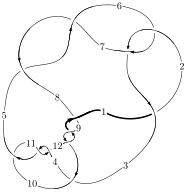
\includegraphics[width=112pt]{../../../GIT/diagram.site/Diagrams/png/1445_12a_0644.png}\\
\ \ \ A knot diagram\footnotemark}&
\allowdisplaybreaks
\textbf{Linearized knot diagam} \\
\cline{2-2}
 &
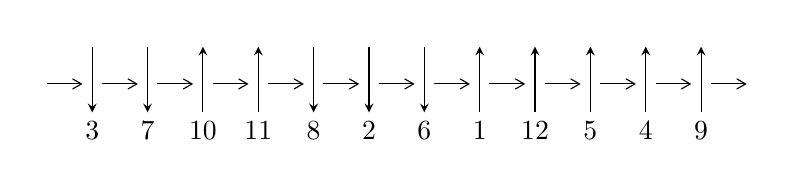
\begin{tikzpicture}[x=20pt, y=17pt]
	% nodes
	\node (C0) at (0, 0) {};
	\node (C1) at (1, 0) {};
	\node (C1U) at (1, +1) {};
	\node (C1D) at (1, -1) {3};

	\node (C2) at (2, 0) {};
	\node (C2U) at (2, +1) {};
	\node (C2D) at (2, -1) {7};

	\node (C3) at (3, 0) {};
	\node (C3U) at (3, +1) {};
	\node (C3D) at (3, -1) {10};

	\node (C4) at (4, 0) {};
	\node (C4U) at (4, +1) {};
	\node (C4D) at (4, -1) {11};

	\node (C5) at (5, 0) {};
	\node (C5U) at (5, +1) {};
	\node (C5D) at (5, -1) {8};

	\node (C6) at (6, 0) {};
	\node (C6U) at (6, +1) {};
	\node (C6D) at (6, -1) {2};

	\node (C7) at (7, 0) {};
	\node (C7U) at (7, +1) {};
	\node (C7D) at (7, -1) {6};

	\node (C8) at (8, 0) {};
	\node (C8U) at (8, +1) {};
	\node (C8D) at (8, -1) {1};

	\node (C9) at (9, 0) {};
	\node (C9U) at (9, +1) {};
	\node (C9D) at (9, -1) {12};

	\node (C10) at (10, 0) {};
	\node (C10U) at (10, +1) {};
	\node (C10D) at (10, -1) {5};

	\node (C11) at (11, 0) {};
	\node (C11U) at (11, +1) {};
	\node (C11D) at (11, -1) {4};

	\node (C12) at (12, 0) {};
	\node (C12U) at (12, +1) {};
	\node (C12D) at (12, -1) {9};
	\node (C13) at (13, 0) {};

	% arrows
	\draw[->,>={angle 60}]
	(C0) edge (C1) (C1) edge (C2) (C2) edge (C3) (C3) edge (C4) (C4) edge (C5) (C5) edge (C6) (C6) edge (C7) (C7) edge (C8) (C8) edge (C9) (C9) edge (C10) (C10) edge (C11) (C11) edge (C12) (C12) edge (C13) ;	\draw[->,>=stealth]
	(C1U) edge (C1D) (C2U) edge (C2D) (C3D) edge (C3U) (C4D) edge (C4U) (C5U) edge (C5D) (C6U) edge (C6D) (C7U) edge (C7D) (C8D) edge (C8U) (C9D) edge (C9U) (C10D) edge (C10U) (C11D) edge (C11U) (C12D) edge (C12U) ;
	\end{tikzpicture} \\
\hhline{~~} \\& 
\textbf{Solving Sequence} \\ \cline{2-2} 
 &
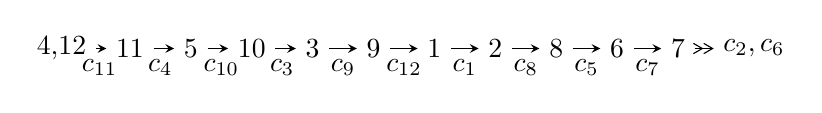
\begin{tikzpicture}[x=22pt, y=7pt]
	% node
	\node (A0) at (-1/8, 0) {4,12};
	\node (A1) at (1, 0) {11};
	\node (A2) at (2, 0) {5};
	\node (A3) at (3, 0) {10};
	\node (A4) at (4, 0) {3};
	\node (A5) at (5, 0) {9};
	\node (A6) at (6, 0) {1};
	\node (A7) at (7, 0) {2};
	\node (A8) at (8, 0) {8};
	\node (A9) at (9, 0) {6};
	\node (A10) at (10, 0) {7};
	\node (C1) at (1/2, -1) {$c_{11}$};
	\node (C2) at (3/2, -1) {$c_{4}$};
	\node (C3) at (5/2, -1) {$c_{10}$};
	\node (C4) at (7/2, -1) {$c_{3}$};
	\node (C5) at (9/2, -1) {$c_{9}$};
	\node (C6) at (11/2, -1) {$c_{12}$};
	\node (C7) at (13/2, -1) {$c_{1}$};
	\node (C8) at (15/2, -1) {$c_{8}$};
	\node (C9) at (17/2, -1) {$c_{5}$};
	\node (C10) at (19/2, -1) {$c_{7}$};
	\node (A11) at (45/4, 0) {$c_{2},c_{6}$};

	% edge
	\draw[->,>=stealth]	
	(A0) edge (A1) (A1) edge (A2) (A2) edge (A3) (A3) edge (A4) (A4) edge (A5) (A5) edge (A6) (A6) edge (A7) (A7) edge (A8) (A8) edge (A9) (A9) edge (A10) ;
	\draw[->>,>={angle 60}]	
	(A10) edge (A11);
\end{tikzpicture} \\ 

\end{tabular} \\

\footnotetext{
The image of knot diagram is generated by the software ``\textbf{Draw programme}" developed by Andrew Bartholomew(\url{http://www.layer8.co.uk/maths/draw/index.htm\#Running-draw}), where we modified some parts for our purpose(\url{https://github.com/CATsTAILs/LinksPainter}).
}\phantom \\ \newline 
\centering \textbf{Ideals for irreducible components\footnotemark of $X_{\text{par}}$} 
 
\begin{align*}
I^u_{1}&=\langle 
u^{56}- u^{55}+\cdots-2 u^2+1\rangle \\
\\
\end{align*}
\raggedright * 1 irreducible components of $\dim_{\mathbb{C}}=0$, with total 56 representations.\\
\footnotetext{All coefficients of polynomials are rational numbers. But the coefficients are sometimes approximated in decimal forms when there is not enough margin.}
\newpage
\renewcommand{\arraystretch}{1}
\centering \section*{I. $I^u_{1}= \langle u^{56}- u^{55}+\cdots-2 u^2+1 \rangle$}
\flushleft \textbf{(i) Arc colorings}\\
\begin{tabular}{m{7pt} m{180pt} m{7pt} m{180pt} }
\flushright $a_{4}=$&$\begin{pmatrix}0\\u\end{pmatrix}$ \\
\flushright $a_{12}=$&$\begin{pmatrix}1\\0\end{pmatrix}$ \\
\flushright $a_{11}=$&$\begin{pmatrix}1\\u^2\end{pmatrix}$ \\
\flushright $a_{5}=$&$\begin{pmatrix}u\\u^3+u\end{pmatrix}$ \\
\flushright $a_{10}=$&$\begin{pmatrix}u^2+1\\u^4+2 u^2\end{pmatrix}$ \\
\flushright $a_{3}=$&$\begin{pmatrix}- u^5-2 u^3- u\\- u^7-3 u^5-2 u^3+u\end{pmatrix}$ \\
\flushright $a_{9}=$&$\begin{pmatrix}- u^4- u^2+1\\u^4+2 u^2\end{pmatrix}$ \\
\flushright $a_{1}=$&$\begin{pmatrix}u^8+3 u^6+u^4-2 u^2+1\\- u^8-4 u^6-4 u^4\end{pmatrix}$ \\
\flushright $a_{2}=$&$\begin{pmatrix}u^{20}+9 u^{18}+\cdots-3 u^2+1\\u^{22}+10 u^{20}+\cdots-10 u^4+u^2\end{pmatrix}$ \\
\flushright $a_{8}=$&$\begin{pmatrix}- u^{12}-5 u^{10}-7 u^8+2 u^4-3 u^2+1\\u^{12}+6 u^{10}+12 u^8+8 u^6+u^4+2 u^2\end{pmatrix}$ \\
\flushright $a_{6}=$&$\begin{pmatrix}- u^{27}-12 u^{25}+\cdots-12 u^5+7 u^3\\u^{27}+13 u^{25}+\cdots- u^3+u\end{pmatrix}$ \\
\flushright $a_{7}=$&$\begin{pmatrix}- u^{42}-19 u^{40}+\cdots-3 u^2+1\\u^{42}+20 u^{40}+\cdots+6 u^4+u^2\end{pmatrix}$\\&\end{tabular}
\flushleft \textbf{(ii) Obstruction class $= -1$}\\~\\
\flushleft \textbf{(iii) Cusp Shapes $= -4 u^{55}+4 u^{54}+\cdots+16 u+2$}\\~\\
\newpage\renewcommand{\arraystretch}{1}
\flushleft \textbf{(iv) u-Polynomials at the component}\newline \\
\begin{tabular}{m{50pt}|m{274pt}}
Crossings & \hspace{64pt}u-Polynomials at each crossing \\
\hline $$\begin{aligned}c_{1},c_{5},c_{7}\end{aligned}$$&$\begin{aligned}
&u^{56}+15 u^{55}+\cdots+4 u+1
\end{aligned}$\\
\hline $$\begin{aligned}c_{2},c_{6}\end{aligned}$$&$\begin{aligned}
&u^{56}- u^{55}+\cdots-2 u^2+1
\end{aligned}$\\
\hline $$\begin{aligned}c_{3}\end{aligned}$$&$\begin{aligned}
&u^{56}+u^{55}+\cdots+202 u+65
\end{aligned}$\\
\hline $$\begin{aligned}c_{4},c_{10},c_{11}\end{aligned}$$&$\begin{aligned}
&u^{56}- u^{55}+\cdots-2 u^2+1
\end{aligned}$\\
\hline $$\begin{aligned}c_{8},c_{9},c_{12}\end{aligned}$$&$\begin{aligned}
&u^{56}+7 u^{55}+\cdots+16 u+1
\end{aligned}$\\
\hline
\end{tabular}\\~\\
\newpage\renewcommand{\arraystretch}{1}
\flushleft \textbf{(v) Riley Polynomials at the component}\newline \\
\begin{tabular}{m{50pt}|m{274pt}}
Crossings & \hspace{64pt}Riley Polynomials at each crossing \\
\hline $$\begin{aligned}c_{1},c_{5},c_{7}\end{aligned}$$&$\begin{aligned}
&y^{56}+53 y^{55}+\cdots+28 y+1
\end{aligned}$\\
\hline $$\begin{aligned}c_{2},c_{6}\end{aligned}$$&$\begin{aligned}
&y^{56}-15 y^{55}+\cdots-4 y+1
\end{aligned}$\\
\hline $$\begin{aligned}c_{3}\end{aligned}$$&$\begin{aligned}
&y^{56}+25 y^{55}+\cdots+239476 y+4225
\end{aligned}$\\
\hline $$\begin{aligned}c_{4},c_{10},c_{11}\end{aligned}$$&$\begin{aligned}
&y^{56}+53 y^{55}+\cdots-4 y+1
\end{aligned}$\\
\hline $$\begin{aligned}c_{8},c_{9},c_{12}\end{aligned}$$&$\begin{aligned}
&y^{56}+57 y^{55}+\cdots+220 y+1
\end{aligned}$\\
\hline
\end{tabular}\\~\\
\newpage\flushleft \textbf{(vi) Complex Volumes and Cusp Shapes}
$$\begin{array}{c|c|c}  
\text{Solutions to }I^u_{1}& \I (\text{vol} + \sqrt{-1}CS) & \text{Cusp shape}\\
 \hline 
\begin{aligned}
u &= \phantom{-}0.020209 + 1.098890 I\end{aligned}
 & \phantom{-}3.96215 + 3.06271 I & \phantom{-0.000000 } 0 \\ \hline\begin{aligned}
u &= \phantom{-}0.020209 - 1.098890 I\end{aligned}
 & \phantom{-}3.96215 - 3.06271 I & \phantom{-0.000000 } 0 \\ \hline\begin{aligned}
u &= \phantom{-}0.686155 + 0.430676 I\end{aligned}
 & -0.39671 + 10.08050 I & \phantom{-}1.51974 - 8.22030 I \\ \hline\begin{aligned}
u &= \phantom{-}0.686155 - 0.430676 I\end{aligned}
 & -0.39671 - 10.08050 I & \phantom{-}1.51974 + 8.22030 I \\ \hline\begin{aligned}
u &= \phantom{-}0.665754 + 0.458645 I\end{aligned}
 & -7.13653 + 5.26062 I & -3.80676 - 6.87867 I \\ \hline\begin{aligned}
u &= \phantom{-}0.665754 - 0.458645 I\end{aligned}
 & -7.13653 - 5.26062 I & -3.80676 + 6.87867 I \\ \hline\begin{aligned}
u &= \phantom{-}0.641196 + 0.486930 I\end{aligned}
 & -7.24731 - 0.92940 I & -4.28257 + 0.58840 I \\ \hline\begin{aligned}
u &= \phantom{-}0.641196 - 0.486930 I\end{aligned}
 & -7.24731 + 0.92940 I & -4.28257 - 0.58840 I \\ \hline\begin{aligned}
u &= \phantom{-}0.611386 + 0.518123 I\end{aligned}
 & -0.73492 - 5.76075 I & \phantom{-}0.62706 + 2.25622 I \\ \hline\begin{aligned}
u &= \phantom{-}0.611386 - 0.518123 I\end{aligned}
 & -0.73492 + 5.76075 I & \phantom{-}0.62706 - 2.25622 I \\ \hline\begin{aligned}
u &= -0.678468 + 0.424262 I\end{aligned}
 & \phantom{-}0.23798 - 3.99471 I & \phantom{-}2.63926 + 3.39930 I \\ \hline\begin{aligned}
u &= -0.678468 - 0.424262 I\end{aligned}
 & \phantom{-}0.23798 + 3.99471 I & \phantom{-}2.63926 - 3.39930 I \\ \hline\begin{aligned}
u &= -0.599558 + 0.509189 I\end{aligned}
 & -0.103709 - 0.253528 I & \phantom{-}1.72073 + 2.79096 I \\ \hline\begin{aligned}
u &= -0.599558 - 0.509189 I\end{aligned}
 & -0.103709 + 0.253528 I & \phantom{-}1.72073 - 2.79096 I \\ \hline\begin{aligned}
u &= -0.637539 + 0.456579 I\end{aligned}
 & -4.01617 - 2.09773 I & \phantom{-}2.12497 + 3.25564 I \\ \hline\begin{aligned}
u &= -0.637539 - 0.456579 I\end{aligned}
 & -4.01617 + 2.09773 I & \phantom{-}2.12497 - 3.25564 I \\ \hline\begin{aligned}
u &= \phantom{-}0.060580 + 1.263240 I\end{aligned}
 & -2.45362 + 1.67355 I & \phantom{-0.000000 } 0 \\ \hline\begin{aligned}
u &= \phantom{-}0.060580 - 1.263240 I\end{aligned}
 & -2.45362 - 1.67355 I & \phantom{-0.000000 } 0 \\ \hline\begin{aligned}
u &= \phantom{-}0.219710 + 1.317140 I\end{aligned}
 & \phantom{-}1.91877 + 2.82951 I & \phantom{-0.000000 } 0 \\ \hline\begin{aligned}
u &= \phantom{-}0.219710 - 1.317140 I\end{aligned}
 & \phantom{-}1.91877 - 2.82951 I & \phantom{-0.000000 } 0 \\ \hline\begin{aligned}
u &= \phantom{-}0.141123 + 1.328370 I\end{aligned}
 & -3.43887 + 2.43530 I & \phantom{-0.000000 } 0 \\ \hline\begin{aligned}
u &= \phantom{-}0.141123 - 1.328370 I\end{aligned}
 & -3.43887 - 2.43530 I & \phantom{-0.000000 } 0 \\ \hline\begin{aligned}
u &= -0.225186 + 1.328010 I\end{aligned}
 & \phantom{-}1.60628 - 8.97008 I & \phantom{-0.000000 } 0 \\ \hline\begin{aligned}
u &= -0.225186 - 1.328010 I\end{aligned}
 & \phantom{-}1.60628 + 8.97008 I & \phantom{-0.000000 } 0 \\ \hline\begin{aligned}
u &= -0.632474 + 0.159551 I\end{aligned}
 & \phantom{-}6.26180 - 5.86038 I & \phantom{-}7.46913 + 7.08001 I \\ \hline\begin{aligned}
u &= -0.632474 - 0.159551 I\end{aligned}
 & \phantom{-}6.26180 + 5.86038 I & \phantom{-}7.46913 - 7.08001 I \\ \hline\begin{aligned}
u &= \phantom{-}0.629195 + 0.140167 I\end{aligned}
 & \phantom{-}6.46439 - 0.24804 I & \phantom{-}8.24330 - 1.61547 I \\ \hline\begin{aligned}
u &= \phantom{-}0.629195 - 0.140167 I\end{aligned}
 & \phantom{-}6.46439 + 0.24804 I & \phantom{-}8.24330 + 1.61547 I \\ \hline\begin{aligned}
u &= -0.178389 + 1.364910 I\end{aligned}
 & -5.35134 - 5.59825 I & \phantom{-0.000000 } 0 \\ \hline\begin{aligned}
u &= -0.178389 - 1.364910 I\end{aligned}
 & -5.35134 + 5.59825 I & \phantom{-0.000000 } 0\\
 \hline 
 \end{array}$$\newpage$$\begin{array}{c|c|c}  
\text{Solutions to }I^u_{1}& \I (\text{vol} + \sqrt{-1}CS) & \text{Cusp shape}\\
 \hline 
\begin{aligned}
u &= -0.038003 + 0.620037 I\end{aligned}
 & \phantom{-}4.15248 + 2.99392 I & \phantom{-}1.86170 - 2.59085 I \\ \hline\begin{aligned}
u &= -0.038003 - 0.620037 I\end{aligned}
 & \phantom{-}4.15248 - 2.99392 I & \phantom{-}1.86170 + 2.59085 I \\ \hline\begin{aligned}
u &= -0.103732 + 1.385290 I\end{aligned}
 & -6.60466 - 0.87132 I & \phantom{-0.000000 } 0 \\ \hline\begin{aligned}
u &= -0.103732 - 1.385290 I\end{aligned}
 & -6.60466 + 0.87132 I & \phantom{-0.000000 } 0 \\ \hline\begin{aligned}
u &= -0.014943 + 1.409750 I\end{aligned}
 & -1.92248 + 2.81822 I & \phantom{-0.000000 } 0 \\ \hline\begin{aligned}
u &= -0.014943 - 1.409750 I\end{aligned}
 & -1.92248 - 2.81822 I & \phantom{-0.000000 } 0 \\ \hline\begin{aligned}
u &= -0.528451 + 0.222220 I\end{aligned}
 & -0.34320 - 3.02564 I & \phantom{-}1.79724 + 9.78051 I \\ \hline\begin{aligned}
u &= -0.528451 - 0.222220 I\end{aligned}
 & -0.34320 + 3.02564 I & \phantom{-}1.79724 - 9.78051 I \\ \hline\begin{aligned}
u &= -0.24877 + 1.47151 I\end{aligned}
 & -5.88112 - 7.38178 I & \phantom{-0.000000 } 0 \\ \hline\begin{aligned}
u &= -0.24877 - 1.47151 I\end{aligned}
 & -5.88112 + 7.38178 I & \phantom{-0.000000 } 0 \\ \hline\begin{aligned}
u &= -0.22908 + 1.47605 I\end{aligned}
 & -10.25770 - 5.26519 I & \phantom{-0.000000 } 0 \\ \hline\begin{aligned}
u &= -0.22908 - 1.47605 I\end{aligned}
 & -10.25770 + 5.26519 I & \phantom{-0.000000 } 0 \\ \hline\begin{aligned}
u &= \phantom{-}0.25090 + 1.47509 I\end{aligned}
 & -6.5513 + 13.5024 I & \phantom{-0.000000 } 0 \\ \hline\begin{aligned}
u &= \phantom{-}0.25090 - 1.47509 I\end{aligned}
 & -6.5513 - 13.5024 I & \phantom{-0.000000 } 0 \\ \hline\begin{aligned}
u &= -0.20488 + 1.48243 I\end{aligned}
 & -6.53709 - 3.16674 I & \phantom{-0.000000 } 0 \\ \hline\begin{aligned}
u &= -0.20488 - 1.48243 I\end{aligned}
 & -6.53709 + 3.16674 I & \phantom{-0.000000 } 0 \\ \hline\begin{aligned}
u &= \phantom{-}0.23824 + 1.48207 I\end{aligned}
 & -13.4144 + 8.5605 I & \phantom{-0.000000 } 0 \\ \hline\begin{aligned}
u &= \phantom{-}0.23824 - 1.48207 I\end{aligned}
 & -13.4144 - 8.5605 I & \phantom{-0.000000 } 0 \\ \hline\begin{aligned}
u &= \phantom{-}0.20573 + 1.48896 I\end{aligned}
 & -7.23525 - 2.80491 I & \phantom{-0.000000 } 0 \\ \hline\begin{aligned}
u &= \phantom{-}0.20573 - 1.48896 I\end{aligned}
 & -7.23525 + 2.80491 I & \phantom{-0.000000 } 0 \\ \hline\begin{aligned}
u &= \phantom{-}0.22358 + 1.48669 I\end{aligned}
 & -13.63780 + 2.21952 I & \phantom{-0.000000 } 0 \\ \hline\begin{aligned}
u &= \phantom{-}0.22358 - 1.48669 I\end{aligned}
 & -13.63780 - 2.21952 I & \phantom{-0.000000 } 0 \\ \hline\begin{aligned}
u &= \phantom{-}0.480726 + 0.076119 I\end{aligned}
 & \phantom{-}0.967130 + 0.223343 I & \phantom{-}10.08613 - 1.09515 I \\ \hline\begin{aligned}
u &= \phantom{-}0.480726 - 0.076119 I\end{aligned}
 & \phantom{-}0.967130 - 0.223343 I & \phantom{-}10.08613 + 1.09515 I \\ \hline\begin{aligned}
u &= -0.255017 + 0.348068 I\end{aligned}
 & -1.263520 + 0.558795 I & -4.83816 - 0.54247 I \\ \hline\begin{aligned}
u &= -0.255017 - 0.348068 I\end{aligned}
 & -1.263520 - 0.558795 I & -4.83816 + 0.54247 I\\
 \hline 
 \end{array}$$\newpage
\newpage\renewcommand{\arraystretch}{1}
\centering \section*{ II. u-Polynomials}
\begin{tabular}{m{50pt}|m{274pt}}
Crossings & \hspace{64pt}u-Polynomials at each crossing \\
\hline $$\begin{aligned}c_{1},c_{5},c_{7}\end{aligned}$$&$\begin{aligned}
&u^{56}+15 u^{55}+\cdots+4 u+1
\end{aligned}$\\
\hline $$\begin{aligned}c_{2},c_{6}\end{aligned}$$&$\begin{aligned}
&u^{56}- u^{55}+\cdots-2 u^2+1
\end{aligned}$\\
\hline $$\begin{aligned}c_{3}\end{aligned}$$&$\begin{aligned}
&u^{56}+u^{55}+\cdots+202 u+65
\end{aligned}$\\
\hline $$\begin{aligned}c_{4},c_{10},c_{11}\end{aligned}$$&$\begin{aligned}
&u^{56}- u^{55}+\cdots-2 u^2+1
\end{aligned}$\\
\hline $$\begin{aligned}c_{8},c_{9},c_{12}\end{aligned}$$&$\begin{aligned}
&u^{56}+7 u^{55}+\cdots+16 u+1
\end{aligned}$\\
\hline
\end{tabular}\newpage\renewcommand{\arraystretch}{1}
\centering \section*{ III. Riley Polynomials}
\begin{tabular}{m{50pt}|m{274pt}}
Crossings & \hspace{64pt}Riley Polynomials at each crossing \\
\hline $$\begin{aligned}c_{1},c_{5},c_{7}\end{aligned}$$&$\begin{aligned}
&y^{56}+53 y^{55}+\cdots+28 y+1
\end{aligned}$\\
\hline $$\begin{aligned}c_{2},c_{6}\end{aligned}$$&$\begin{aligned}
&y^{56}-15 y^{55}+\cdots-4 y+1
\end{aligned}$\\
\hline $$\begin{aligned}c_{3}\end{aligned}$$&$\begin{aligned}
&y^{56}+25 y^{55}+\cdots+239476 y+4225
\end{aligned}$\\
\hline $$\begin{aligned}c_{4},c_{10},c_{11}\end{aligned}$$&$\begin{aligned}
&y^{56}+53 y^{55}+\cdots-4 y+1
\end{aligned}$\\
\hline $$\begin{aligned}c_{8},c_{9},c_{12}\end{aligned}$$&$\begin{aligned}
&y^{56}+57 y^{55}+\cdots+220 y+1
\end{aligned}$\\
\hline
\end{tabular}
\vskip 2pc
\end{document}